% TerraScope -- final research paper (IEEEtran conference format).
% Build: pdflatex TerraScope_Research_Paper; bibtex is not needed (the reference list is inline); run pdflatex twice.
\documentclass[conference]{IEEEtran}
\usepackage{cite}
\usepackage{amsmath,amssymb}
\usepackage{graphicx}
\usepackage{booktabs}
\usepackage{url}
\usepackage{textcomp}
\graphicspath{{figures-final/}}

\begin{document}

\title{Crop Health Monitoring Using NDVI and Sentinel-2 Imagery: A Field-Level Audit of an NDVI Decline Rule on Indian Smallholder Fields}

\author{
\IEEEauthorblockN{Tushar Singh}
\IEEEauthorblockA{\textit{School of Computer Science and Engineering}\\
\textit{IILM University}\\
Greater Noida, India\\
tushar.singh.cs28@iilm.edu}
\and
\IEEEauthorblockN{Anurodh Singh}
\IEEEauthorblockA{\textit{School of Computer Science and Engineering}\\
\textit{IILM University}\\
Greater Noida, India\\
anurodh.singh.cs28@iilm.edu}
\and
\IEEEauthorblockN{Vansh Thakur}
\IEEEauthorblockA{\textit{School of Computer Science and Engineering}\\
\textit{IILM University}\\
Greater Noida, India\\
vansh.thakur.cs28@iilm.edu}
\and
\IEEEauthorblockN{Sahil Sharma}
\IEEEauthorblockA{\textit{School of Computer Science and Engineering}\\
\textit{IILM University}\\
Greater Noida, India\\
sahil.sharma.cs28@iilm.edu}
}

\maketitle

\begin{abstract}
Satellite crop-monitoring dashboards often turn the Normalized Difference Vegetation Index (NDVI) into a single health value, even when the image is cloudy, old or covers only part of a small field. We present TerraScope, a field-level monitoring prototype that computes NDVI from Sentinel-2 L2A imagery, masks clouds with the scene classification layer, accepts a measurement only when at least 70\% of the field and 10 pixels are clear, and raises a visit request when NDVI falls by 0.10 or more within 30 days. We ask whether the measurement layer is reliable on small Indian fields and whether the decline rule separates problem fields from healthy ones. On 31,104 field-images from 584 Telangana fields the cloud mask agreed with the independent Cloud Score+ reference (Spearman $\rho = 0.838$), and only 0.3\% of accepted images were strongly unclear. Replayed on 3,700 survey-labelled fields of the Telangana Crop Health Challenge, the decline rule alerted on 79.9\% of problem fields and 78.6\% of healthy fields (AUC 0.498, balanced accuracy 50.6\%, macro-F1 0.32), in every one of seven crops. On real series the rule fired on 12.2\% of healthy mid-season image pairs and detected a 0.30 NDVI drop over 30\% of a field in only 48.1\% of pairs. A MobileNetV2 leaf-photo classifier trained from scratch on 15,519 Uttar Pradesh field photographs reached 94.7\% accuracy (macro-F1 0.946) and kept at least 90.1\% under seven phone-photo degradations. Two case studies from the deployed app show that nearly equal declines ($-0.31$ and $-0.32$) are judged by the crop calendar, not by the change itself. The measurement layer is sound, but a fixed NDVI decline is a reason to inspect a field, not a stress detector.
\end{abstract}

\begin{IEEEkeywords}
crop health monitoring, NDVI, Sentinel-2, cloud masking, precision agriculture, smallholder farming, decision rules, leaf disease classification.
\end{IEEEkeywords}

\section{Introduction}
Most farms in India are small: in the Agriculture Census 2015--16, small and marginal holdings (below 2\,ha) made up 86.21\% of all operational holdings, and the average holding was 1.08\,ha \cite{r1}. Small farms also dominate worldwide \cite{r2}. The Sentinel-2 mission images land at 10\,m resolution in the red and near-infrared bands about every five days \cite{r3}, which is enough to follow a field of a few hundred square metres without visiting it. The usual measure is $\mathrm{NDVI} = (\rho_{\mathrm{NIR}} - \rho_{\mathrm{red}})/(\rho_{\mathrm{NIR}} + \rho_{\mathrm{red}})$, which is high for dense green canopy and low for bare soil \cite{r4,r5}, and reviews of agricultural remote sensing treat it as a proxy for canopy vigour \cite{r6,r7}.

\textbf{Problem statement.} Turning NDVI into advice for a small field involves choices that most dashboards hide. Clouds and shadows corrupt pixels, a small field may have only a handful of clear pixels, and the same overpass can arrive in two overlapping tiles with different values. In our data one 3.57\,ha field measured NDVI 0.246 in tile 43RGK and 0.317 in tile 43RGL on the same day, a gap of 0.071 that is close to the 0.10 change used to raise alerts. A fall in NDVI is also often read as crop stress, although it can come from harvest, senescence or irrigation. A wrong ``all clear'' can cost a harvest, and a wrong alarm costs a farmer's trust.

\textbf{Research questions.} We therefore ask: (RQ1) does Sentinel-2 cloud masking with a whole-field coverage gate give field-level NDVI that agrees with an independent cloud reference on small Indian fields; (RQ2) does a fixed decline rule (a fall of 0.10 within 30 days) separate survey-labelled problem fields from healthy ones; and (RQ3) how robust is a leaf-photo classifier trained on Indian field photographs to the photo problems of phone use?

\textbf{Contributions.} The contributions are measurements, not new methods:
\begin{enumerate}
\renewcommand{\labelenumi}{(\roman{enumi})}
\item On 31,104 field-images from 584 Telangana fields, the scene-classification mask agreed with Cloud Score+ ($\rho = 0.838$); 0.3\% of accepted images were strongly unclear, and removing edge pixels changed at most 1.0\% of decline decisions (RQ1).
\item On 3,700 labelled fields, the decline rule had no discriminative power (AUC 0.498, balanced accuracy 50.6\%), and this held in all seven crops and five field-size classes (RQ2).
\item On 19,141 real healthy image pairs, the rule had a false-trigger floor of 12.2\%, and an injected 0.30 drop was detected four times above that floor only when about 30\% of the field was affected (RQ2).
\item A MobileNetV2 trained from scratch on PLDD-UP reached 94.7\% accuracy and macro-F1 0.946, and a robustness check showed that the run with the highest clean score (96.7\%) fell to 70.0\% under low colour, while the chosen run stayed at or above 90.1\% (RQ3).
\item Two case studies from the deployed app, with screenshots and measurements, show that two almost equal declines ($-0.31$ and $-0.32$) are reported as normal or as a problem depending only on whether a harvest date was entered, and that monsoon months can have no clear picture at all.
\end{enumerate}
Section~II reviews related work, Section~III describes the data and methods, Section~IV reports the results and the app case studies, Section~V discusses them, and Section~VI gives limitations; full per-class results are in the appendix.

\section{Related Work}
\subsection{Vegetation indices and cloud masking}
NDVI contrasts near-infrared and red reflectance \cite{r4,r5}; moisture indices such as NDMI use the short-wave infrared band \cite{r8}. Sentinel-2 Level-2A products are produced by Sen2Cor, which also outputs a scene classification layer (SCL) that labels cloud, shadow, cirrus and snow \cite{r9}. Against reference masks, Sen2Cor reached about 84\% overall accuracy, below MAJA and Fmask at about 90--91\% \cite{r10}, and an international intercomparison found good agreement on thick cloud but not on thin cloud \cite{r11}. These studies score pixels over whole scenes; they do not report how many field-level decisions change, which we measure against Cloud Score+ \cite{r12}.

\subsection{Crop-stress detection from satellite data}
Recent work learns stress-sensitive indices instead of using a fixed NDVI threshold. Seralathan and Shirly Edward \cite{r13} used reinforcement learning to build a vegetation index from Sentinel-2 and mobile imagery for rice in Tamil Nadu and reported 89.4\% overall accuracy and an F1-score of 0.88. Such results depend on labels that are matched in time to the images. Random cross-validation also overstates accuracy for spatially structured data \cite{r14}, and information that leaks from the target into the features gives optimistic scores \cite{r15}. We therefore test a simple, transparent rule against independent survey labels rather than training on them.

\subsection{Leaf-image disease classification}
Convolutional networks reach 99.35\% on the PlantVillage laboratory images, but Mohanty \emph{et al.} reported that accuracy fell to 31.4\% on leaf images from other sources \cite{r16}, and Barbedo describes the factors behind this gap \cite{r17}. On potato, Bhavani and Chalapathi \cite{r18} reported 93.2\% for a MobileNetV2 baseline on PlantVillage-derived potato images, and field datasets taken in uncontrolled conditions are now available \cite{r19,r20}. We train on field photographs from Uttar Pradesh and test robustness explicitly.

\subsection{Existing monitoring tools}
Table~\ref{tab:tools} compares how three widely used tools document cloud handling and alerts. The comparison uses public documentation only; we did not run these tools, and ``not documented'' does not mean ``absent''.

\begin{table}[t]
\caption{Documented cloud handling in related tools (Nov. 2026)}
\label{tab:tools}
\centering
\footnotesize
\begin{tabular}{@{}p{1.55cm}p{3.7cm}p{1.9cm}@{}}
\toprule
Tool & Cloud handling (documented) & Change alerts \\
\midrule
OneSoil \cite{r21} & Cloud, shadow and snow detected; NDVI only where clear & Not documented \\
EOSDA Crop Monitoring \cite{r22} & User cloud threshold; images above 50\% cloud hidden by default & Abnormal NDVI drop (vendor) \\
Copernicus Browser \cite{r23} & Scene-level cloud filter (default 30\%) & None \\
TerraScope (ours) & Per-pixel SCL mask; whole-field gate ($\geq$70\%, $\geq$10\,px) & Decline rule on comparable pairs \\
\bottomrule
\end{tabular}
\end{table}

\section{Data and Methods}
\subsection{Data sources}
Table~\ref{tab:data} lists every dataset with its version, licence and use. Imagery is Sentinel-2 L2A surface reflectance, read from the open Earth Search catalogue in the prototype and from the Earth Engine collection \texttt{COPERNICUS/S2\_SR\_HARMONIZED} \cite{r24} for the experiments. NASA POWER weather is used for context only \cite{r25}. None of the datasets in Table~\ref{tab:data} is redistributed with this work.

\begin{table}[t]
\caption{Datasets, versions and licences}
\label{tab:data}
\centering
\footnotesize
\begin{tabular}{@{}p{1.7cm}p{2.5cm}p{1.0cm}p{1.1cm}@{}}
\toprule
Dataset & Version / identifier & Licence & Use \\
\midrule
Sentinel-2 L2A \cite{r3} & \texttt{COPERNICUS/\allowbreak S2\_SR\_\allowbreak HARMONIZED} & Open & All NDVI \\
Telangana Crop Health Challenge \cite{r26} & Zindi, competition 8 Nov 2024--9 Feb 2025; Train.csv & CC BY-SA 4.0 & Evaluation only \\
PLDD-UP \cite{r20} & Mendeley Data V1, doi:10.17632/\allowbreak 3j4nfkvp2n.1 & CC BY 4.0 & Leaf model \\
AgriFieldNet \cite{r27} & v1.0, doi:10.34911/\allowbreak rdnt.wu92p1 & CC BY 4.0 & Crop-type control \\
NASA POWER \cite{r25} & Daily, district level & Open & Rainfall check \\
\bottomrule
\end{tabular}
\end{table}

The Telangana training file holds 7,888 fields labelled Healthy (6,506), Pests (485), Diseased (474) or Stressed (423), with sowing and harvest dates, crop and irrigation source, for seven crops in the 2022--2024 seasons \cite{r26}. Fields under 0.3\,ha were excluded because they cannot meet the 10-pixel gate, which left 3,725 fields (median 0.58\,ha); 3,700 of them received at least one decided assessment (661 problem, 3,039 healthy). The labels are season-level survey categories without a date, not expert visits matched to image dates.

\subsection{Index computation and coverage gate}
Reflectance scale and offset are taken from scene metadata (the $-0.1$ offset of processing baseline 04.00 and later is applied), and the engine refuses to guess a scale. Pixels in SCL classes 0--3 and 8--11 (no data, saturated, dark, cloud shadow, cloud, cirrus, snow) are excluded \cite{r9}. NDVI is computed from bands B8 and B4. An image is accepted when at least 70\% of the field and at least 10 pixels are clear, with the whole field polygon as the coverage denominator. Each observation is stored with its scene, tile, boundary revision and calculation method (Fig.~\ref{fig:pipeline}).

\begin{figure}[t]
\centering
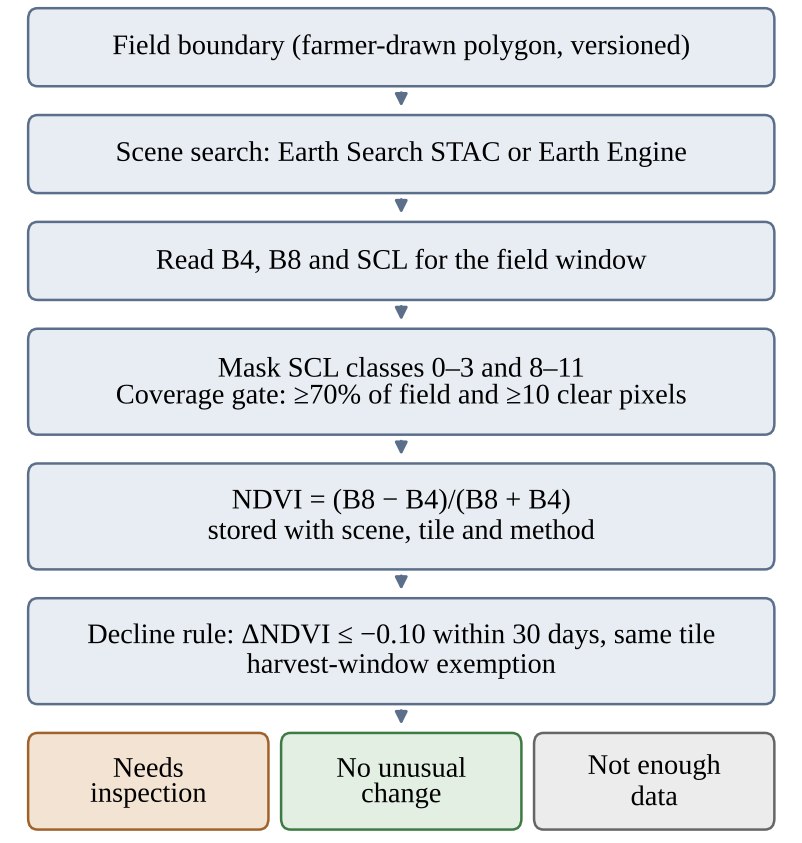
\includegraphics[width=0.8\columnwidth]{fig1_pipeline.png}
\caption{Processing pipeline of the TerraScope prototype, from field boundary to one of three assessment states.}
\label{fig:pipeline}
\end{figure}

\subsection{Decision rule}
A fall of 0.10 or more between two accepted images at most 30 days apart, from the same tile and calculation method, returns ``needs inspection''. From 30 days before to 45 days after a recorded harvest date, the fall is reported as expected ripening or harvest. If no accepted image is recent enough or images are not comparable, the state is ``not enough data''. These thresholds are initial product settings and were not tuned on the evaluation labels.

\subsection{Evaluation protocol}
\textit{Measurement layer (RQ1).} For a size-stratified sample of 584 fields we summarised every in-season image (31,104 field-images on the primary tile) and compared the SCL clear share with Cloud Score+ (clear if cs\_cdf $\geq$ 0.6) \cite{r12}. An accepted image is \emph{strongly unclear} if its mean Cloud Score+ is below 0.30. Edge effects were measured by shrinking each polygon by 10\,m.

\textit{Rule replay (RQ2).} The application's own code was replayed on every accepted image between sowing and harvest, 109,596 assessments in total. A field counts as alerted if the replay says ``visit'' at least once in the season. Problem fields (Pests, Diseased, Stressed) are the positive class. We report recall, specificity, precision, balanced accuracy, macro-averaged precision, recall and F1 over the two classes, and the AUC of the per-field share of alerting assessments with a 95\% bootstrap interval; other intervals are Wilson intervals. To measure sensitivity on real noise, we took 19,141 comparable mid-season pairs (40--80\% of the season) from healthy fields and subtracted $0.30\cdot f$ from each change, which is the field-mean effect of a 0.30 drop over a share $f$ of the field.

\textit{Further checks.} A gradient-boosted model \cite{r28} was trained on NDVI, red-edge and moisture curves, weather and field-record columns for 3,644 fields; a peer check scored each field against same-crop neighbours; and, as a control, the same features were used to predict crop type. Recorded harvest dates and NASA POWER rainfall were used as label-free evidence.

\textit{Leaf photos (RQ3).} A MobileNetV2 \cite{r29} was trained from random initialisation, to avoid unclear licences of pretrained weights, on PLDD-UP \cite{r20}: 15,519 photographs in three classes (Healthy 4,600, Early Blight 4,803, Late Blight 6,116). Exact and near-duplicate groups (SHA-256 and 64-bit difference hash) were kept within one split. Test photos were degraded in seven ways (dim light, glare, blur, JPEG quality 15, off-centre crop, $40^{\circ}$ rotation, low colour). Selection criteria for each run were committed before training.

\section{Results}
\subsection{Measurement layer (RQ1)}
The SCL mask and Cloud Score+ agreed closely ($\rho = 0.838$; mean absolute difference 0.084 in clear share). The gate accepted 63.9\% of all field-images, and of the images rejected by the gate, the reference called 17.4\% at least 90\% clear, so the gate is conservative rather than permissive. Only 0.3\% of accepted images (60) were strongly unclear, and NDVI under the SCL mask differed from NDVI under both masks by more than 0.05 in 0.3\% of accepted images. Among images with any valid pixel, the gate accepted 94.0--96.8\% across field-size classes. A one-pixel edge ring holds 52\% of the pixels of a 0.3--0.4\,ha field, but removing it changed the decline decision for at most 1.0\% of pairs. Only 1.5\% of ``all clear'' decisions (1,094 of 72,882) rested on thin evidence (an image below 85\% coverage or 30 pixels).

Fig.~\ref{fig:masks} shows the layer on one real 3.09\,ha field (20 October 2023, tile 44QLD). The SCL mask kept 45\% of the field and Cloud Score+ kept 53\%; both removed the same cloud bank, so the image was rejected by the gate (below 70\%) rather than averaged over cloud.

\begin{figure}[t]
\centering
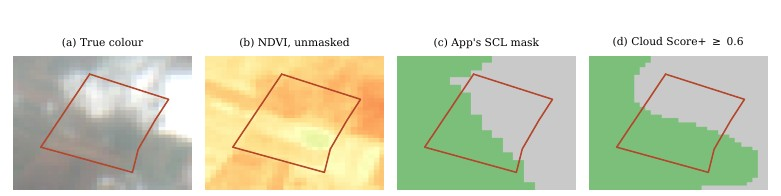
\includegraphics[width=\columnwidth]{fig2_masks.jpeg}
\caption{One real field (3.09\,ha, 20 Oct 2023, tile 44QLD): (a) true colour, (b) unmasked NDVI, (c) the app's SCL mask (45\% clear), (d) Cloud Score+ $\geq$ 0.6 (53\% clear). Grey: masked; green: kept; red: field boundary.}
\label{fig:masks}
\end{figure}

\subsection{Decline-rule replay (RQ2)}
Of the 109,596 assessments, 90.4\% were ``no unusual change'', 7.5\% ``needs inspection'' and 2.2\% ``not enough data''. Table~\ref{tab:confusion} gives the season-level confusion matrix and the macro-averaged metrics. Alerts appeared on 79.9\% of problem fields and 78.6\% of healthy fields, so an alert carried no information about the label. The precision of 18.1\% equals the share of problem fields (17.9\%). The result held in each crop and size class (Appendix, Tables A1 and A2): for example, cotton alerted on 74.7\% of problem and 73.4\% of healthy fields.

\begin{table}[t]
\caption{Season-level replay of the decline rule (3,700 fields)}
\label{tab:confusion}
\centering
\footnotesize
\begin{tabular}{@{}lccc@{}}
\toprule
 & Alerted & Never alerted & Total \\
\midrule
Problem fields & 528 & 133 & 661 \\
Healthy fields & 2,389 & 650 & 3,039 \\
Recall / specificity & 79.9\% & 21.4\% & \\
Precision / NPV & 18.1\% & 83.0\% & \\
Balanced accuracy & \multicolumn{3}{c}{50.6\%} \\
Macro P / R / F1 & \multicolumn{3}{c}{0.506 / 0.506 / 0.318} \\
AUC (95\% interval) & \multicolumn{3}{c}{0.498 (0.472--0.517)} \\
\bottomrule
\end{tabular}

\vspace{2pt}
{\scriptsize Positive class: problem (Pests, Diseased, Stressed). NPV: negative predictive value. Macro averages are the unweighted mean over the two classes.}
\end{table}

Fig.~\ref{fig:maize} shows a typical false alert. A maize field of 1.81\,ha, labelled healthy in the survey, was followed over two crop cycles. Every accepted picture passed the gate, and the rule fired at both harvest drops, the steepest real declines in the series. No harvest date was recorded for this field in the app, so the exemption could not apply.

\begin{figure}[t]
\centering
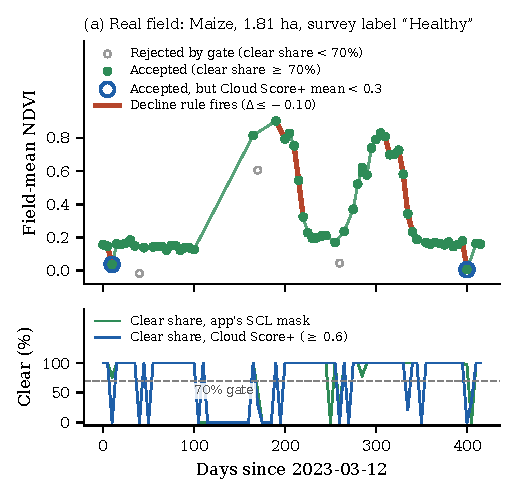
\includegraphics[width=\columnwidth]{fig3_maize_series.pdf}
\caption{Real maize field (1.81\,ha, survey label healthy) from 12 Mar 2023. Top: field-mean NDVI; red segments are where the decline rule fires. Bottom: clear share under the SCL mask and Cloud Score+, with the 70\% gate.}
\label{fig:maize}
\end{figure}

Fig.~\ref{fig:sensitivity} shows why. With no injected stress, 12.2\% of healthy mid-season pairs already fired, because ordinary variation is large (median absolute change 0.040, 90th percentile 0.162). The flagged share rose to 28.4\% when 20\% of the field was affected and to 48.1\% at 30\%. On synthetic rasters with independent noise the same rule switched from 0\% to 100\% at about 33\%; real noise turns that step into a gradual curve with a floor of false triggers.

\begin{figure}[t]
\centering
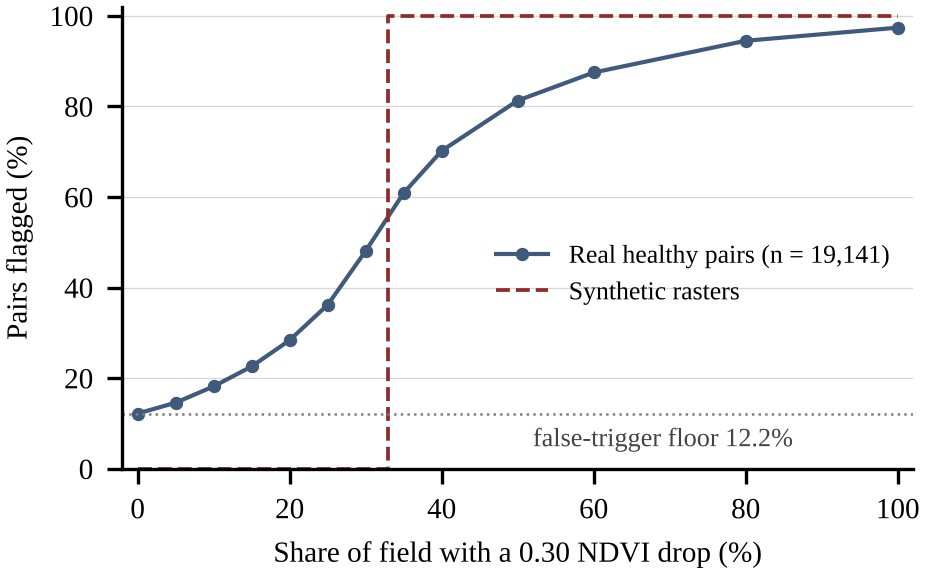
\includegraphics[width=\columnwidth]{fig4_sensitivity.png}
\caption{Share of healthy mid-season image pairs flagged by the decline rule after a 0.30 NDVI drop over part of the field. Real pairs (blue, 19,141 pairs from 1,958 fields) against synthetic rasters (red).}
\label{fig:sensitivity}
\end{figure}

The model-based checks found no signal either: the gradient-boosted model reached AUC 0.48--0.52 and the peer check 0.49--0.51, while the crop-type control reached 77\% accuracy against a 30\% baseline, which shows that the pipeline itself works. Recorded harvest dates agreed with the canopy (NDVI peaked a median of 66 days before harvest), but in the monsoon season declines were more frequent in the wettest rainfall tercile than in the driest (16.1\% against 5.5\% of pairs in rainfed fields), so rainfall gives no support that the rule detects water stress.

\subsection{Comparison with published results}
Table~\ref{tab:compare} places our numbers next to published ones. The published stress result \cite{r13} is a learned index scored against time-matched labels, whereas our rule is fixed and scored against undated survey labels, so the two are not a contest; the comparison shows how far a fixed NDVI threshold is from what learned models report. For leaf photos, our field-photo accuracy is in the range of published potato baselines on laboratory-style images \cite{r18}, and below the PlantVillage figure \cite{r16}, which drops sharply on images from other sources.

\begin{table}[t]
\caption{Comparison with published results}
\label{tab:compare}
\centering
\footnotesize
\begin{tabular}{@{}p{1.55cm}p{1.8cm}p{1.6cm}p{1.6cm}@{}}
\toprule
Work & Data & Method & Result \\
\midrule
Seralathan \& Shirly Edward \cite{r13} & S2 + mobile, rice, Tamil Nadu & Learned index (RL) & OA 89.4\%, F1 0.88 \\
Ours & S2, 3,700 fields, Telangana & Fixed $\Delta$NDVI $\leq -0.10$ & AUC 0.498, bal.\ acc.\ 50.6\% \\
\midrule
Baetens \emph{et al.} \cite{r10} & S2 scenes vs reference masks & Sen2Cor SCL & OA $\approx$ 84\% \\
Ours & 31,104 field-images & SCL vs Cloud Score+ & $\rho$ 0.838; 0.3\% strongly unclear \\
\midrule
Mohanty \emph{et al.} \cite{r16} & PlantVillage lab leaves & CNN & 99.35\%; 31.4\% on other sources \\
Bhavani \& Chalapathi \cite{r18} & PlantVillage-derived potato & MobileNetV2 & 93.2\% \\
Ours & PLDD-UP field photos, UP & MobileNetV2, scratch & 94.7\%, macro-F1 0.946 \\
\bottomrule
\end{tabular}
\end{table}

\subsection{Leaf-photo model (RQ3)}
Run 4 reached 94.7\% test accuracy and macro-F1 0.946, and called 1.4\% of diseased test leaves healthy (20 of 1,394). Run 2 scored higher on clean photos (96.7\%) but lost 18 to 27 points under dim light, blur and low colour (Fig.~\ref{fig:robust}), so the more robust run 4 was kept. With a photo-quality gate and a calibrated ``not sure, retake the photo'' rule, run 4 answered 87.2\% of clean test photos and called a diseased leaf healthy in 0.75\% of answered ones. Full results for all degradations are in Table A3.

\begin{figure}[t]
\centering
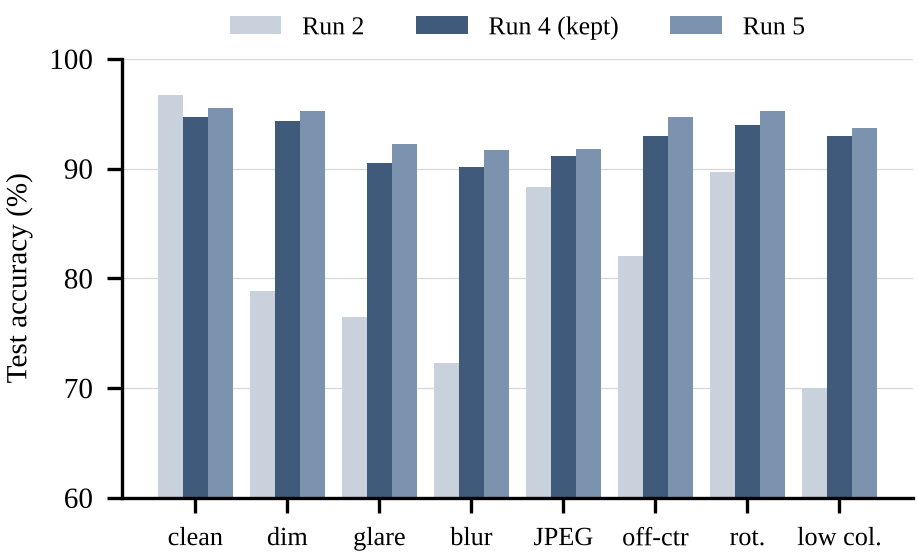
\includegraphics[width=\columnwidth]{fig5_robustness.png}
\caption{Potato leaf-photo test accuracy of three MobileNetV2 runs on clean and degraded photos. Run 2 scored highest on clean photos but fell most under degradation.}
\label{fig:robust}
\end{figure}

Two further results guard against inflated scores. A first rice run scored 100\% because 97\% of its test photos had a near copy in training; after a flip- and rotation-invariant duplicate check the score fell to 94.8\%, and the 100\% result was voided. A crop-type model on AgriFieldNet \cite{r27} reached 59.1\% accuracy but macro-F1 of only 0.22 (rice F1 0.11), so it is not usable.

\subsection{Case studies from the running prototype}
The screenshots in Figs.~\ref{fig:caseA}--\ref{fig:caseBmonth} are taken from the deployed TerraScope app on two fields monitored in October and November 2026. They are not part of the labelled evaluation; they show how the rules and measurements behave on live data. Table~\ref{tab:cases} lists the values read from the screens and the changes derived from them.

\textit{Case A: decline after a recorded harvest.} The two-date screen (Fig.~\ref{fig:caseA}) compares 8 and 23 November 2026 on one colour scale ($-0.2$ to 1). Both pictures were 100\% clear (0\% cloud), so the gate accepted them at full coverage. Field-mean NDVI fell from 0.51 to 0.20, a change of $-0.309$ in 15 days, which is three times the 0.10 threshold and 1.9 times the 90th percentile of ordinary change in the replay (0.162). Over the three accepted pictures (Fig.~\ref{fig:caseAseries}) the field went from dense (0.61) to the border of bare soil (0.20), and the map turned from uniform green to uniform red, so the fall affected the whole field rather than a patch. Because the farmer had recorded a harvest date, the change fell inside the harvest window and the app reported the stage as after harvest, with no alarm.

\begin{figure}[t]
\centering
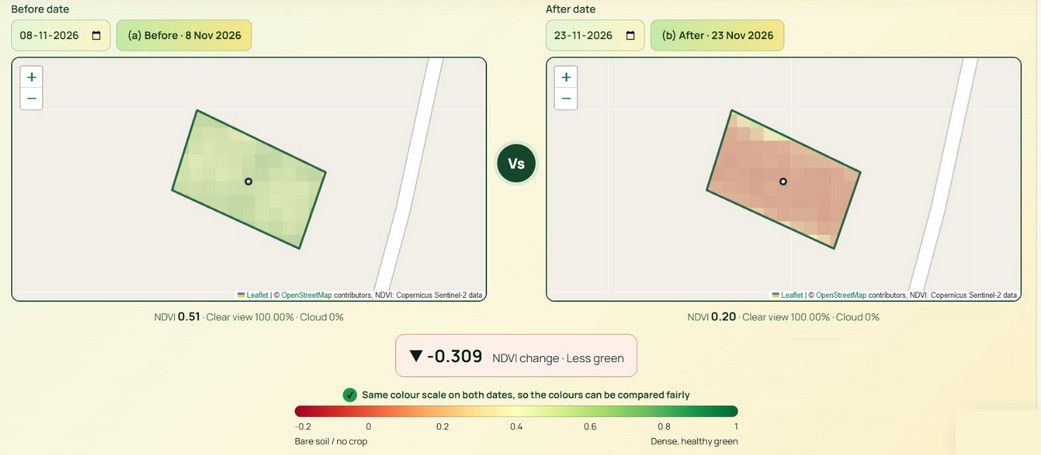
\includegraphics[width=\columnwidth]{fig6_caseA_compare.jpeg}
\caption{Case A, two-date comparison screen of the app. 8 Nov 2026: NDVI 0.51, 100\% clear; 23 Nov 2026: NDVI 0.20, 100\% clear; change $-0.309$. Both maps share one colour scale.}
\label{fig:caseA}
\end{figure}

\begin{figure}[t]
\centering
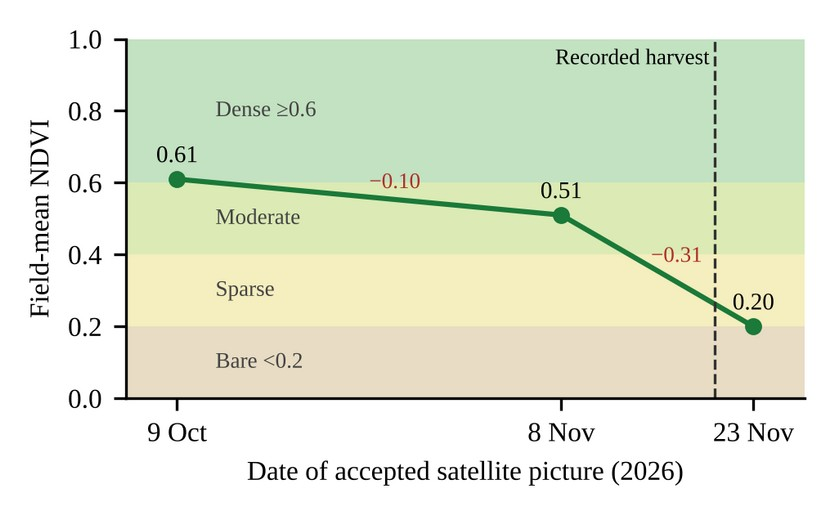
\includegraphics[width=0.85\columnwidth]{fig7_caseA_series.jpeg}
\caption{Case A, NDVI of the three accepted pictures with the greenness bands used by the app and the recorded harvest date.}
\label{fig:caseAseries}
\end{figure}

\textit{Case B: the same kind of decline without a crop calendar.} The field-history screen (Fig.~\ref{fig:caseB}) shows five pictures between 4 October and 13 November 2026, about one every 10 days. NDVI fell from 0.87 to 0.71 in three small steps ($-0.04$, $-0.07$, $-0.05$), each inside the ordinary variation measured in Section~IV-B, and then by $-0.32$ in the last 10 days to 0.39 (sparse or weak green). The total fall since the first picture was $-0.48$. Only the last step crossed the threshold, and the app raised needs inspection. No sowing or harvest date had been entered, so the stage was reported as unknown and the exemption could not be applied.

\begin{figure}[t]
\centering
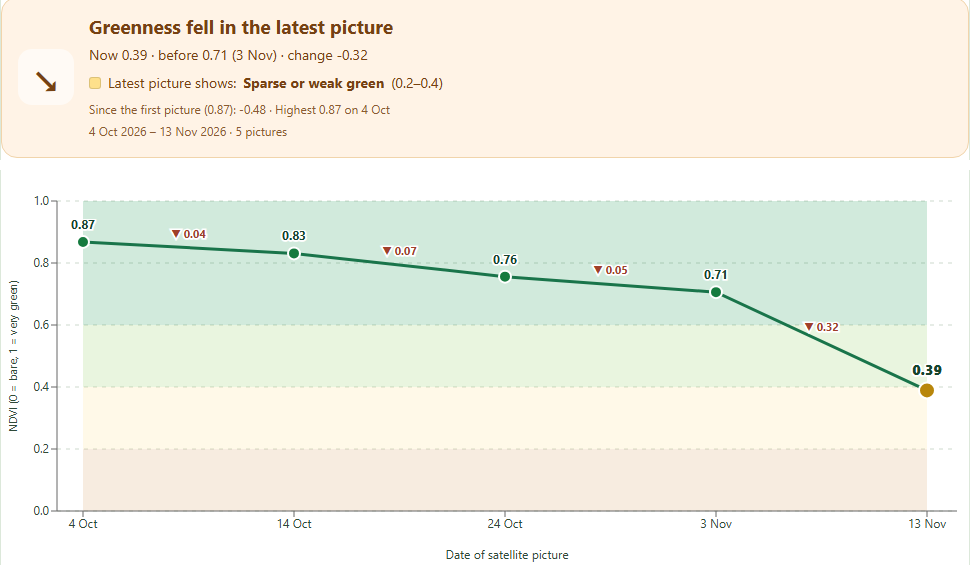
\includegraphics[width=\columnwidth]{fig8_caseB_history.png}
\caption{Case B, field-history screen of the app: alert card and NDVI of five pictures (4 Oct--13 Nov 2026) with the step change between pictures.}
\label{fig:caseB}
\end{figure}

The monthly panel of Case B (Fig.~\ref{fig:caseBmonth}) gives two further measurements. First, August and September 2026 had no clear picture at all, so the monsoon cloud gap is visible on a real field: the series jumps from 0.45 in July to 0.87 in October with nothing in between. Second, the monthly view takes the best picture of each month, so November shows 0.71 although the latest picture is 0.39; a monthly maximum hides a decline that happens within the month, and the alert must come from the picture-level series.

\begin{figure}[t]
\centering
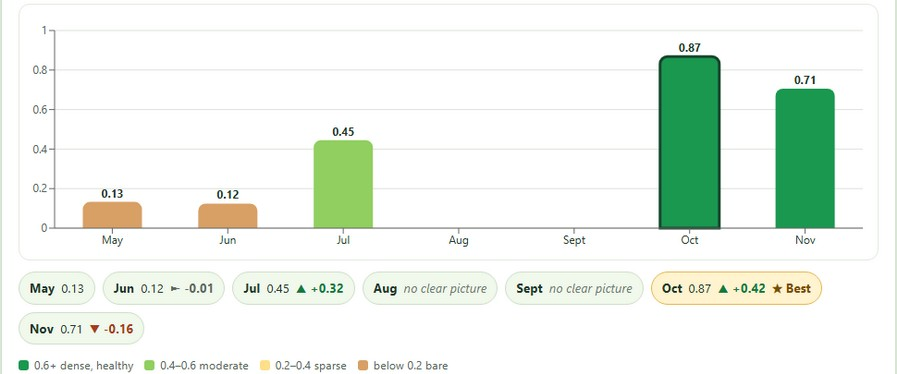
\includegraphics[width=0.9\columnwidth]{fig9_caseB_monthly.jpeg}
\caption{Case B, best NDVI of each month, May--Nov 2026. August and September had no clear picture and are left empty, not guessed.}
\label{fig:caseBmonth}
\end{figure}

\begin{table}[t]
\caption{Measurements from the two app case studies}
\label{tab:cases}
\centering
\footnotesize
\begin{tabular}{@{}p{2.45cm}p{2.5cm}p{2.5cm}@{}}
\toprule
Measure & Case A & Case B \\
\midrule
Accepted pictures (span) & 3 (9 Oct--23 Nov) & 5 (4 Oct--13 Nov) \\
Clear view of compared pictures & 100\%, 0\% cloud & Passed gate ($\geq$ 70\%) \\
First $\to$ latest NDVI & 0.61 $\to$ 0.20 & 0.87 $\to$ 0.39 \\
Total change & $-0.41$ & $-0.48$ \\
Largest step (days) & $-0.309$ (15) & $-0.32$ (10) \\
Largest step / threshold & 3.1$\times$ & 3.2$\times$ \\
Largest step / ordinary p90 & 1.9$\times$ & 2.0$\times$ \\
Latest greenness band & Sparse (border of bare) & Sparse or weak (0.2--0.4) \\
Crop calendar & Harvest date recorded & None entered \\
App state & No alarm (after harvest) & Needs inspection \\
Months without clear picture & --- & Aug, Sep \\
\bottomrule
\end{tabular}

\vspace{2pt}
{\scriptsize Values read from the app screens (Figs.~\ref{fig:caseA}--\ref{fig:caseBmonth}). Ordinary p90: 90th percentile of absolute change between healthy mid-season pairs (0.162, Section~IV-B).}
\end{table}

Read together, the two cases make the main finding of this paper concrete. The two declines are almost the same size ($-0.31$ and $-0.32$) and both are well above the threshold, yet one is reported as normal and the other as a problem, and the only difference is whether the farmer typed in a harvest date. The rule is therefore a calendar check as much as a stress check, which is consistent with the replay, where harvest declines produced most alerts on healthy fields (Fig.~\ref{fig:maize}). Neither case was checked on the ground, so they illustrate the behaviour of the system and do not measure its accuracy.

\section{Discussion}
\textit{The measurement layer holds; the decision layer does not.} RQ1 is answered positively: careful masking and a whole-field denominator give an NDVI value that agrees with an independent reference, and neither residual cloud (0.3\%), edge pixels ($\leq$ 1.0\% of decisions) nor thin evidence (1.5\%) explains the behaviour of the rule. RQ2 is answered negatively: the 0.10 threshold lies inside the ordinary variation of real series, which produces a 12.2\% false-trigger floor, and the strongest genuine decline in these data is the senescence before harvest.

\textit{Why one global threshold is weak.} Our own results show that the meaning of an alert depends on the crop: healthy fields alerted on 94.9\% of Bengal gram fields but on 52.1\% of groundnut fields (Table A1). A single threshold cannot fit both. Per-crop and per-stage expectations, or a per-pixel temporal baseline, are needed, and calibrating them requires dated, verified labels.

\textit{Bounds of the negative result.} The Telangana labels are season-level and undated, and polygon accuracy was not checked, so a noisy label would weaken any rule. Our claim is therefore bounded: the rule as designed cannot be shown to detect survey-labelled problems. We did not tune any threshold on these labels, so the result is an honest out-of-sample test.

\textit{Leaf photos.} RQ3 shows that clean-test accuracy can mislead: the highest-scoring run was the least robust. All photo results come from public datasets of one region and season, and a check on 1,561 unlabelled West Bengal canopy photos showed signs of domain shift, so these are not the accuracy a farmer would see.

\section{Limitations and Future Work}
The thresholds are uncalibrated; the validation labels come from Telangana, not Uttar Pradesh, and do not say when stress occurred; fields under 0.3\,ha cannot be monitored at 10\,m; rainfall is district-level and confounded with season; and Cloud Score+ is a learned score, not hand-labelled truth. The leaf model has not been tested on labelled photos from the app's own fields. Future work will collect 30 to 100 dated, consented field visits labelled by a trained reviewer, recalibrate thresholds per crop and stage, replace the field-mean rule with per-pixel temporal baselines, and add radar imagery for monsoon months.

\section{Conclusion}
TerraScope turns a farmer-drawn boundary into dated, quality-checked NDVI values and separates ``needs inspection'' from ``not enough data''. On 31,104 field-images the cloud mask and coverage gate were reliable. On 3,700 labelled fields a fixed decline of 0.10 within 30 days had no discriminative power (AUC 0.498), and a field-photo leaf model reached 94.7\% while staying robust to phone-photo problems. We therefore make no claim that the system detects crop stress. Until dated, verified labels allow calibration, an NDVI drop in this system means one thing: look at the field.

\section*{Data and Code Availability}
Code, experiment scripts and aggregate results are at \url{https://github.com/tusharsingh-1801/91-CHM} (commit \texttt{efc3200}); a snapshot of the repository is archived at Zenodo (DOI 10.5281/zenodo.24590449). The datasets in Table~\ref{tab:data} are not redistributed and must be obtained from their sources.

\section*{Acknowledgment}
The authors thank their guide, Mr.~Vikas Singh, for his guidance and supervision of this work, and the School of Computer Science and Engineering, IILM University, for its support.

\section*{Appendix: Full Results}
\setcounter{table}{0}
\renewcommand{\thetable}{A\arabic{table}}

\begin{table}[h]
\caption{Decline-rule replay by crop}
\centering
\footnotesize
\begin{tabular}{@{}lcccc@{}}
\toprule
Crop & Fields (P / H) & Alert P & Alert H & Precision \\
\midrule
Cotton & 1,115 (194 / 921) & 74.7\% & 73.4\% & 17.7\% \\
Maize & 692 (116 / 576) & 90.5\% & 88.4\% & 17.1\% \\
Bengal gram & 663 (134 / 529) & 97.0\% & 94.9\% & 20.6\% \\
Groundnut & 442 (77 / 365) & 54.5\% & 52.1\% & 18.1\% \\
Paddy & 327 (54 / 273) & 72.2\% & 80.2\% & 15.1\% \\
Chillies & 306 (45 / 261) & 75.6\% & 77.4\% & 14.4\% \\
Red gram & 155 (41 / 114) & 80.5\% & 79.8\% & 26.6\% \\
All & 3,700 (661 / 3,039) & 79.9\% & 78.6\% & 18.1\% \\
\bottomrule
\end{tabular}

\vspace{2pt}
{\scriptsize P: problem fields; H: healthy fields. Alert: share of fields alerted at least once in the season.}
\end{table}

\begin{table}[h]
\caption{Decline-rule replay by field size}
\centering
\footnotesize
\begin{tabular}{@{}lcccc@{}}
\toprule
Area (ha) & Fields (P / H) & Alert P & Alert H & \begin{tabular}[c]{@{}c@{}}Healthy-pair\\ false trigger\end{tabular} \\
\midrule
0.3--0.4 & 849 (142 / 707) & 76.8\% & 80.1\% & 11.4\% \\
0.4--0.6 & 1,081 (198 / 883) & 79.3\% & 78.5\% & 11.6\% \\
0.6--1.0 & 1,070 (197 / 873) & 83.8\% & 75.5\% & 12.7\% \\
1.0--2.0 & 598 (109 / 489) & 75.2\% & 81.4\% & 13.2\% \\
$\geq$ 2.0 & 102 (15 / 87) & 100.0\% & 83.9\% & 14.8\% \\
\bottomrule
\end{tabular}

\vspace{2pt}
{\scriptsize Last column: share of comparable healthy mid-season image pairs flagged by the rule.}
\end{table}

\begin{table}[h]
\caption{Potato leaf-photo runs under degradation: accuracy / diseased called healthy}
\centering
\footnotesize
\begin{tabular}{@{}lccc@{}}
\toprule
Condition & Run 2 & Run 4 (kept) & Run 5 \\
\midrule
Clean & 96.7\% / 0.5\% & 94.7\% / 1.4\% & 95.5\% / 1.3\% \\
Dim light ($\times$0.5) & 78.8\% / 2.3\% & 94.3\% / 1.7\% & 95.2\% / 1.3\% \\
Glare ($\times$1.7) & 76.5\% / 2.9\% & 90.5\% / 3.6\% & 92.2\% / 2.6\% \\
Blur (radius 3) & 72.3\% / 12.3\% & 90.1\% / 1.9\% & 91.7\% / 2.1\% \\
JPEG (q = 15) & 88.3\% / 6.0\% & 91.1\% / 3.4\% & 91.8\% / 2.3\% \\
Off-centre crop & 82.0\% / 5.4\% & 93.0\% / 2.2\% & 94.7\% / 1.7\% \\
Rotated $40^{\circ}$ & 89.7\% / 2.4\% & 94.0\% / 1.5\% & 95.2\% / 1.2\% \\
Low colour ($\times$0.3) & 70.0\% / 13.4\% & 93.0\% / 2.0\% & 93.7\% / 1.9\% \\
Macro-F1 (clean) & 0.967 & 0.946 & 0.953 \\
\bottomrule
\end{tabular}

\vspace{2pt}
{\scriptsize Run 5 did not meet its pre-declared criteria (gate and ``not sure'' rule), so run 4 remains the candidate.}
\end{table}

\begin{thebibliography}{99}
\bibitem{r1} Ministry of Agriculture and Farmers Welfare, Government of India, ``Agriculture Census 2015--16 (Phase I): Provisional results,'' New Delhi, Oct. 2018.
\bibitem{r2} S. K. Lowder, J. Skoet, and T. Raney, ``The number, size, and distribution of farms, smallholder farms, and family farms worldwide,'' \emph{World Development}, vol. 87, pp. 16--29, 2016.
\bibitem{r3} M. Drusch \emph{et al.}, ``Sentinel-2: ESA's optical high-resolution mission for GMES operational services,'' \emph{Remote Sensing of Environment}, vol. 120, pp. 25--36, 2012.
\bibitem{r4} J. W. Rouse, R. H. Haas, J. A. Schell, and D. W. Deering, ``Monitoring vegetation systems in the Great Plains with ERTS,'' NASA SP-351, 1974.
\bibitem{r5} C. J. Tucker, ``Red and photographic infrared linear combinations for monitoring vegetation,'' \emph{Remote Sensing of Environment}, vol. 8, no. 2, pp. 127--150, 1979.
\bibitem{r6} M. Weiss, F. Jacob, and G. Duveiller, ``Remote sensing for agricultural applications: A meta-review,'' \emph{Remote Sensing of Environment}, vol. 236, 2020.
\bibitem{r7} D. J. Mulla, ``Twenty five years of remote sensing in precision agriculture: Key advances and remaining knowledge gaps,'' \emph{Biosystems Engineering}, vol. 114, no. 4, pp. 358--371, 2013.
\bibitem{r8} B.-C. Gao, ``NDWI---A normalized difference water index for remote sensing of vegetation liquid water from space,'' \emph{Remote Sensing of Environment}, vol. 58, no. 3, pp. 257--266, 1996.
\bibitem{r9} M. Main-Knorn \emph{et al.}, ``Sen2Cor for Sentinel-2,'' in \emph{Proc. SPIE}, vol. 10427, 2017.
\bibitem{r10} L. Baetens, C. Desjardins, and O. Hagolle, ``Validation of Copernicus Sentinel-2 cloud masks obtained from MAJA, Sen2Cor, and FMask processors using reference cloud masks generated with a supervised active learning procedure,'' \emph{Remote Sensing}, vol. 11, no. 4, p. 433, 2019.
\bibitem{r11} S. Skakun \emph{et al.}, ``Cloud Mask Intercomparison eXercise (CMIX): An evaluation of cloud masking algorithms for Landsat 8 and Sentinel-2,'' \emph{Remote Sensing of Environment}, vol. 274, p. 112990, 2022.
\bibitem{r12} V. J. Pasquarella, C. F. Brown, W. Czerwinski, and W. J. Rucklidge, ``Comprehensive quality assessment of optical satellite imagery using weakly supervised video learning,'' in \emph{Proc. IEEE/CVF CVPR Workshops}, 2023, pp. 2125--2135.
\bibitem{r13} P. Seralathan and A. Shirly Edward, ``Reinforcement learning based dynamic vegetation index formulation for rice crop stress detection using satellite and mobile imagery,'' \emph{Scientific Reports}, vol. 16, art. 3447, 2025, doi:10.1038/s41598-025-33386-9.
\bibitem{r14} D. R. Roberts \emph{et al.}, ``Cross-validation strategies for data with temporal, spatial, hierarchical, or phylogenetic structure,'' \emph{Ecography}, vol. 40, no. 8, pp. 913--929, 2017.
\bibitem{r15} S. Kaufman, S. Rosset, C. Perlich, and O. Stitelman, ``Leakage in data mining: Formulation, detection, and avoidance,'' \emph{ACM Trans. Knowledge Discovery from Data}, vol. 6, no. 4, pp. 15:1--15:21, 2012.
\bibitem{r16} S. P. Mohanty, D. P. Hughes, and M. Salath\'e, ``Using deep learning for image-based plant disease detection,'' \emph{Frontiers in Plant Science}, vol. 7, p. 1419, 2016.
\bibitem{r17} J. G. A. Barbedo, ``Factors influencing the use of deep learning for plant disease recognition,'' \emph{Biosystems Engineering}, vol. 172, pp. 84--91, 2018.
\bibitem{r18} G. D. Bhavani and M. M. V. Chalapathi, ``PotatoLeafNet: Two-stage convolutional neural networks for effective potato leaf disease identification and classification,'' \emph{Frontiers in Artificial Intelligence}, vol. 8, art. 1668839, 2026, doi:10.3389/frai.2025.1668839.
\bibitem{r19} N. H. Shabrina \emph{et al.}, ``A novel dataset of potato leaf disease in uncontrolled environment,'' \emph{Data in Brief}, vol. 52, p. 109955, 2024.
\bibitem{r20} P. K. Singh, A. Yadav, D. Yadav, S. Tiwari, and A. Chandel, ``PLDD-UP: Potato leaf disease dataset from Uttar Pradesh, India,'' Mendeley Data, V1, 2026, doi:10.17632/3j4nfkvp2n.1.
\bibitem{r21} OneSoil, ``Why aren't I getting vegetation index updates?,'' OneSoil Help Center, accessed 23 Nov. 2026.
\bibitem{r22} EOS Data Analytics, ``EOSDA Crop Monitoring: User guide and key functions,'' vendor documentation, accessed 23 Nov. 2026.
\bibitem{r23} Copernicus Data Space Ecosystem, ``About the Copernicus Browser,'' documentation, accessed 23 Nov. 2026.
\bibitem{r24} N. Gorelick \emph{et al.}, ``Google Earth Engine: Planetary-scale geospatial analysis for everyone,'' \emph{Remote Sensing of Environment}, vol. 202, pp. 18--27, 2017.
\bibitem{r25} A. H. Sparks, ``nasapower: A NASA POWER global meteorology, surface solar energy and climatology data client for R,'' \emph{J. Open Source Software}, vol. 3, no. 30, p. 1035, 2018.
\bibitem{r26} Zindi, GIZ FAIR Forward, Government of Telangana, and ADeX, ``Telangana Crop Health Challenge,'' competition dataset, 2024--2025, CC BY-SA 4.0.
\bibitem{r27} Radiant Earth Foundation and IDinsight, ``AgriFieldNet Competition Dataset v1.0,'' 2022, doi:10.34911/rdnt.wu92p1.
\bibitem{r28} J. H. Friedman, ``Greedy function approximation: A gradient boosting machine,'' \emph{Annals of Statistics}, vol. 29, no. 5, pp. 1189--1232, 2001.
\bibitem{r29} M. Sandler, A. Howard, M. Zhu, A. Zhmoginov, and L.-C. Chen, ``MobileNetV2: Inverted residuals and linear bottlenecks,'' in \emph{Proc. IEEE/CVF CVPR}, 2018, pp. 4510--4520.
\end{thebibliography}

\end{document}
